\section{Resultados}
De la figura 4 podemos analizar que de una entrada dada de 40 selecciones se puede sugerir un conjunto de propiedades con una K de 7 probamos distintos valores de K para refinar la consulta y obtener resultados con características similares a la entrada de datos.
Sin embargo al utilizaar este algoritmo utilizamos una función de normalización de los datos buscando que las propiedades consideradas en la misma escala, se afecta el resultado del clasificador.


\begin{figure}[h]
\centering
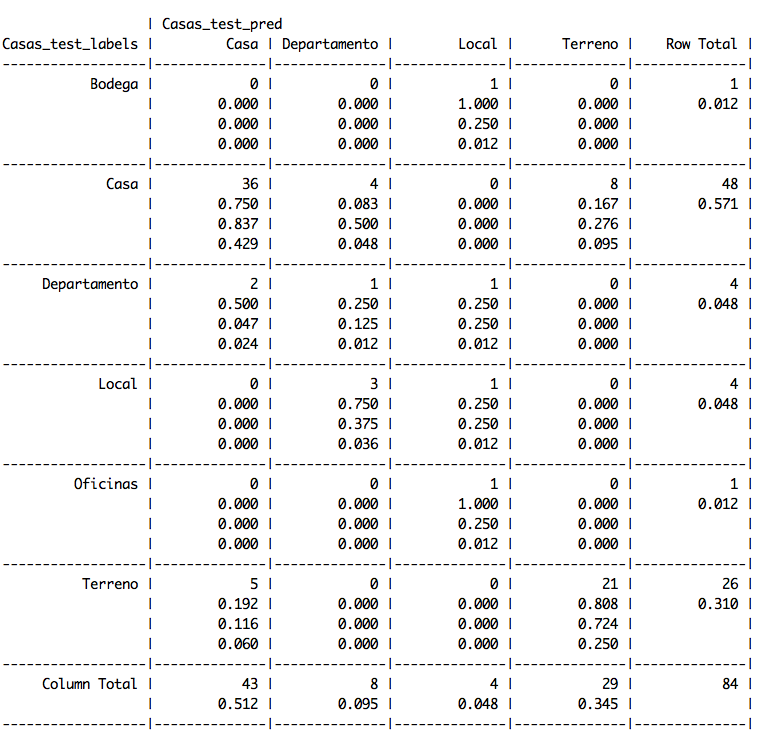
\includegraphics[width=0.9\textwidth]{ModeloPredictivo.png}
\caption{Propiedades recomendadas según la selección del Usuario}
\end{figure}